\chapter{Implementation}

In this chapter, the process of implementation will be covered, starting by the architecture and the tools to the results and how everything fits together.

\section{Tools}
\subsection{React JS}

\begin{wrapfigure}[10]{r}{3cm}
	\vspace{-10pt}
	
\includegraphics[width=3cm]{images/chapter3/logo-react-js.png}
	\vspace{-10pt}
	\caption{{\footnotesize React JS framework logo}}
\end{wrapfigure}

React (also known as React.js or ReactJS) is a free and open-source front-end JavaScript library\cite{ReactJavaScriptLibrary} for building user interfaces or UI components. It is maintained by Facebook and a community of individual developers and companies.\cite{ReactMakingFaster} React can be used as a base in the development of single-page or mobile applications. However, React is only concerned with state management and rendering that state to the DOM, so creating React applications usually requires the use of additional libraries for routing, as well as certain client-side functionality.

\subsection{Web3.js}

There are a few different aspects to developing blockchain applications with Ethereum:

\begin{itemize}
\item \textbf{Smart contract development} - writing code that gets deployed to the blockchain with the Solidity programming language.
\item \textbf{Developing websites or clients that interact with the blockchain} - writing code that reads and writes data from the blockchain with smart contracts.
\end{itemize}

\begin{wrapfigure}[9]{r}{3cm}
	\vspace{-10pt}
	
\includegraphics[width=3cm]{images/chapter3/web3.jpeg}
	\vspace{-10pt}
	\caption{{\footnotesize Web3 logo}}
\end{wrapfigure}

Web3.js enables you to fulfill the second responsibility: developing clients that interact with The Etherem Blockchain. It is a collection of libraries that allow you to perform actions like send Ether from one account to another, read and write data from smart contracts, create smart contracts, and so much more.

Web3.js communicates to The Ethereum Blockchain with JSON RPC, which stands for "Remote Procedure Call" protocol. Ethereum is a peer-to-peer network of nodes that stores a copy of all the data and code on the blockchain. Web3.js allows us to make requests to an individual Ethereum node with JSON RPC in order to read and write data to the network\cite{mccubbinIntroWeb3Js}.

\subsection{Ganache}

\begin{wrapfigure}[11]{r}{2.5cm}
	\vspace{-10pt}
	
\includegraphics[width=2.5cm]{images/chapter3/ganache-logo-dark.png}
	\vspace{-10pt}
	\caption{{\footnotesize Ganache Logo}}
\end{wrapfigure}

Ganache is a personal blockchain for rapid Ethereum and Corda distributed application development. You can use Ganache across the entire development cycle; enabling you to develop, deploy, and test your dApps in a safe and deterministic environment.

Ganache comes in two flavors: a UI and CLI. Ganache UI is a desktop application supporting both Ethereum and Corda technology. The command-line tool, ganache-cli (formerly known as the TestRPC), is available for Ethereum development. Prefer using the command-line? This documentation will focus only on the UI flavor of Ganache. Please see the Ganache CLI Readme for command-line documentation.

All versions of Ganache are available for Windows, Mac, and Linux\cite{GanacheOverviewDocumentation}.

\begin{figure}[H]
	\centering
		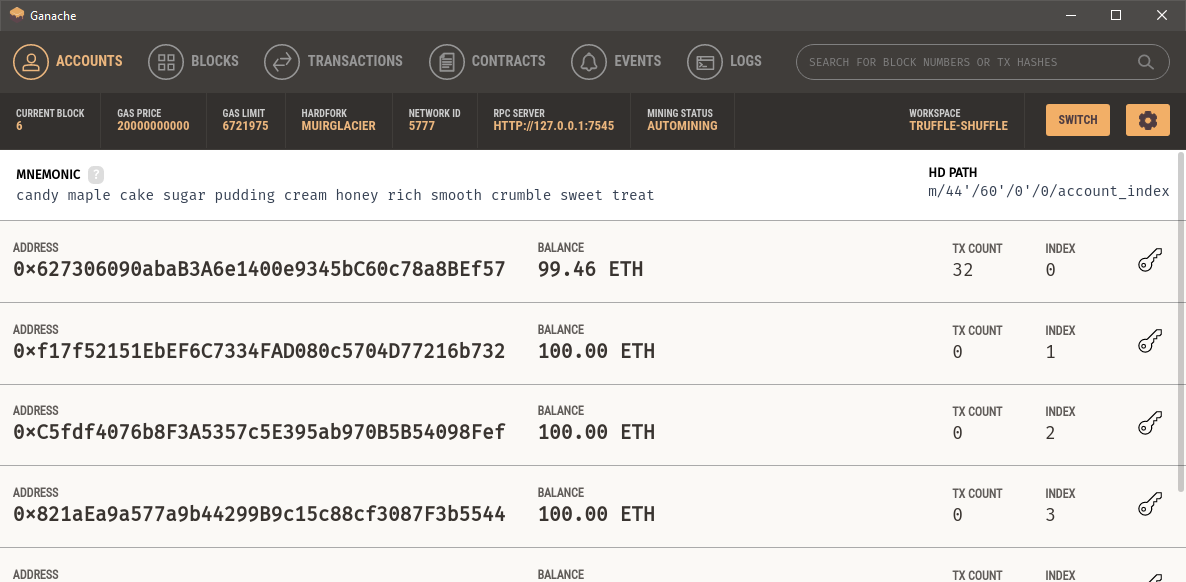
\includegraphics[width=10cm]{images/chapter3/ganache-window.png}
		\caption{{\footnotesize Ganache GUI}}
\end{figure}

\subsection{MetaMask}

\begin{wrapfigure}[10]{r}{2.5cm}
	\vspace{-10pt}
	
\includegraphics[width=2.5cm]{images/chapter3/metamask-logo.png}
	\vspace{-10pt}
	\caption{{\footnotesize MetaMask Logo}}
\end{wrapfigure}

MetaMask is a software cryptocurrency wallet used to interact with the Ethereum blockchain.\cite{schroederCryptoWalletMetaMask2020} It allows users to access their Ethereum wallet through a browser extension or mobile app, which can then be used to interact with decentralized applications.

MetaMask allows users to store and manage account keys, broadcast transactions, send and receive Ethereum-based cryptocurrencies and tokens, and securely connect to decentralized applications through a compatible web browser or the mobile app's built-in browser.[3][4]

The application includes an integrated service for exchanging Ethereum tokens by aggregating several decentralized exchanges (DEXs) to find the best exchange rate. This feature, branded as MetaMask Swaps, charges a service fee of 0.875\% of the transaction amount\cite{schroederCryptoWalletMetaMask2021}.

\begin{figure}[h]
	\centering
		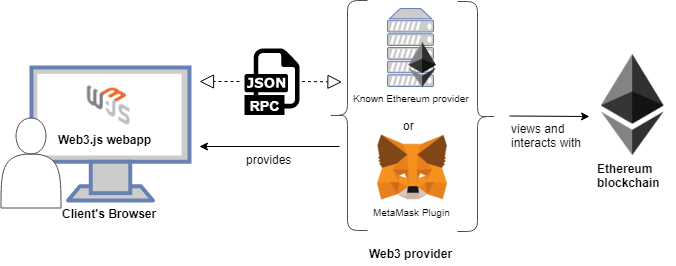
\includegraphics[width=12cm]{images/chapter3/web3-architecture.png}
		\caption{{\footnotesize architecture of a client application interaction with a blockchain network using Web3 and MetaMask}}
\end{figure}

\section{System Design}

In this section we introduce our proposed voting system that aims to solve some of the barriers that traditional voting systems have.

\subsection{Architecture}

\begin{figure}[H]
	\centering
		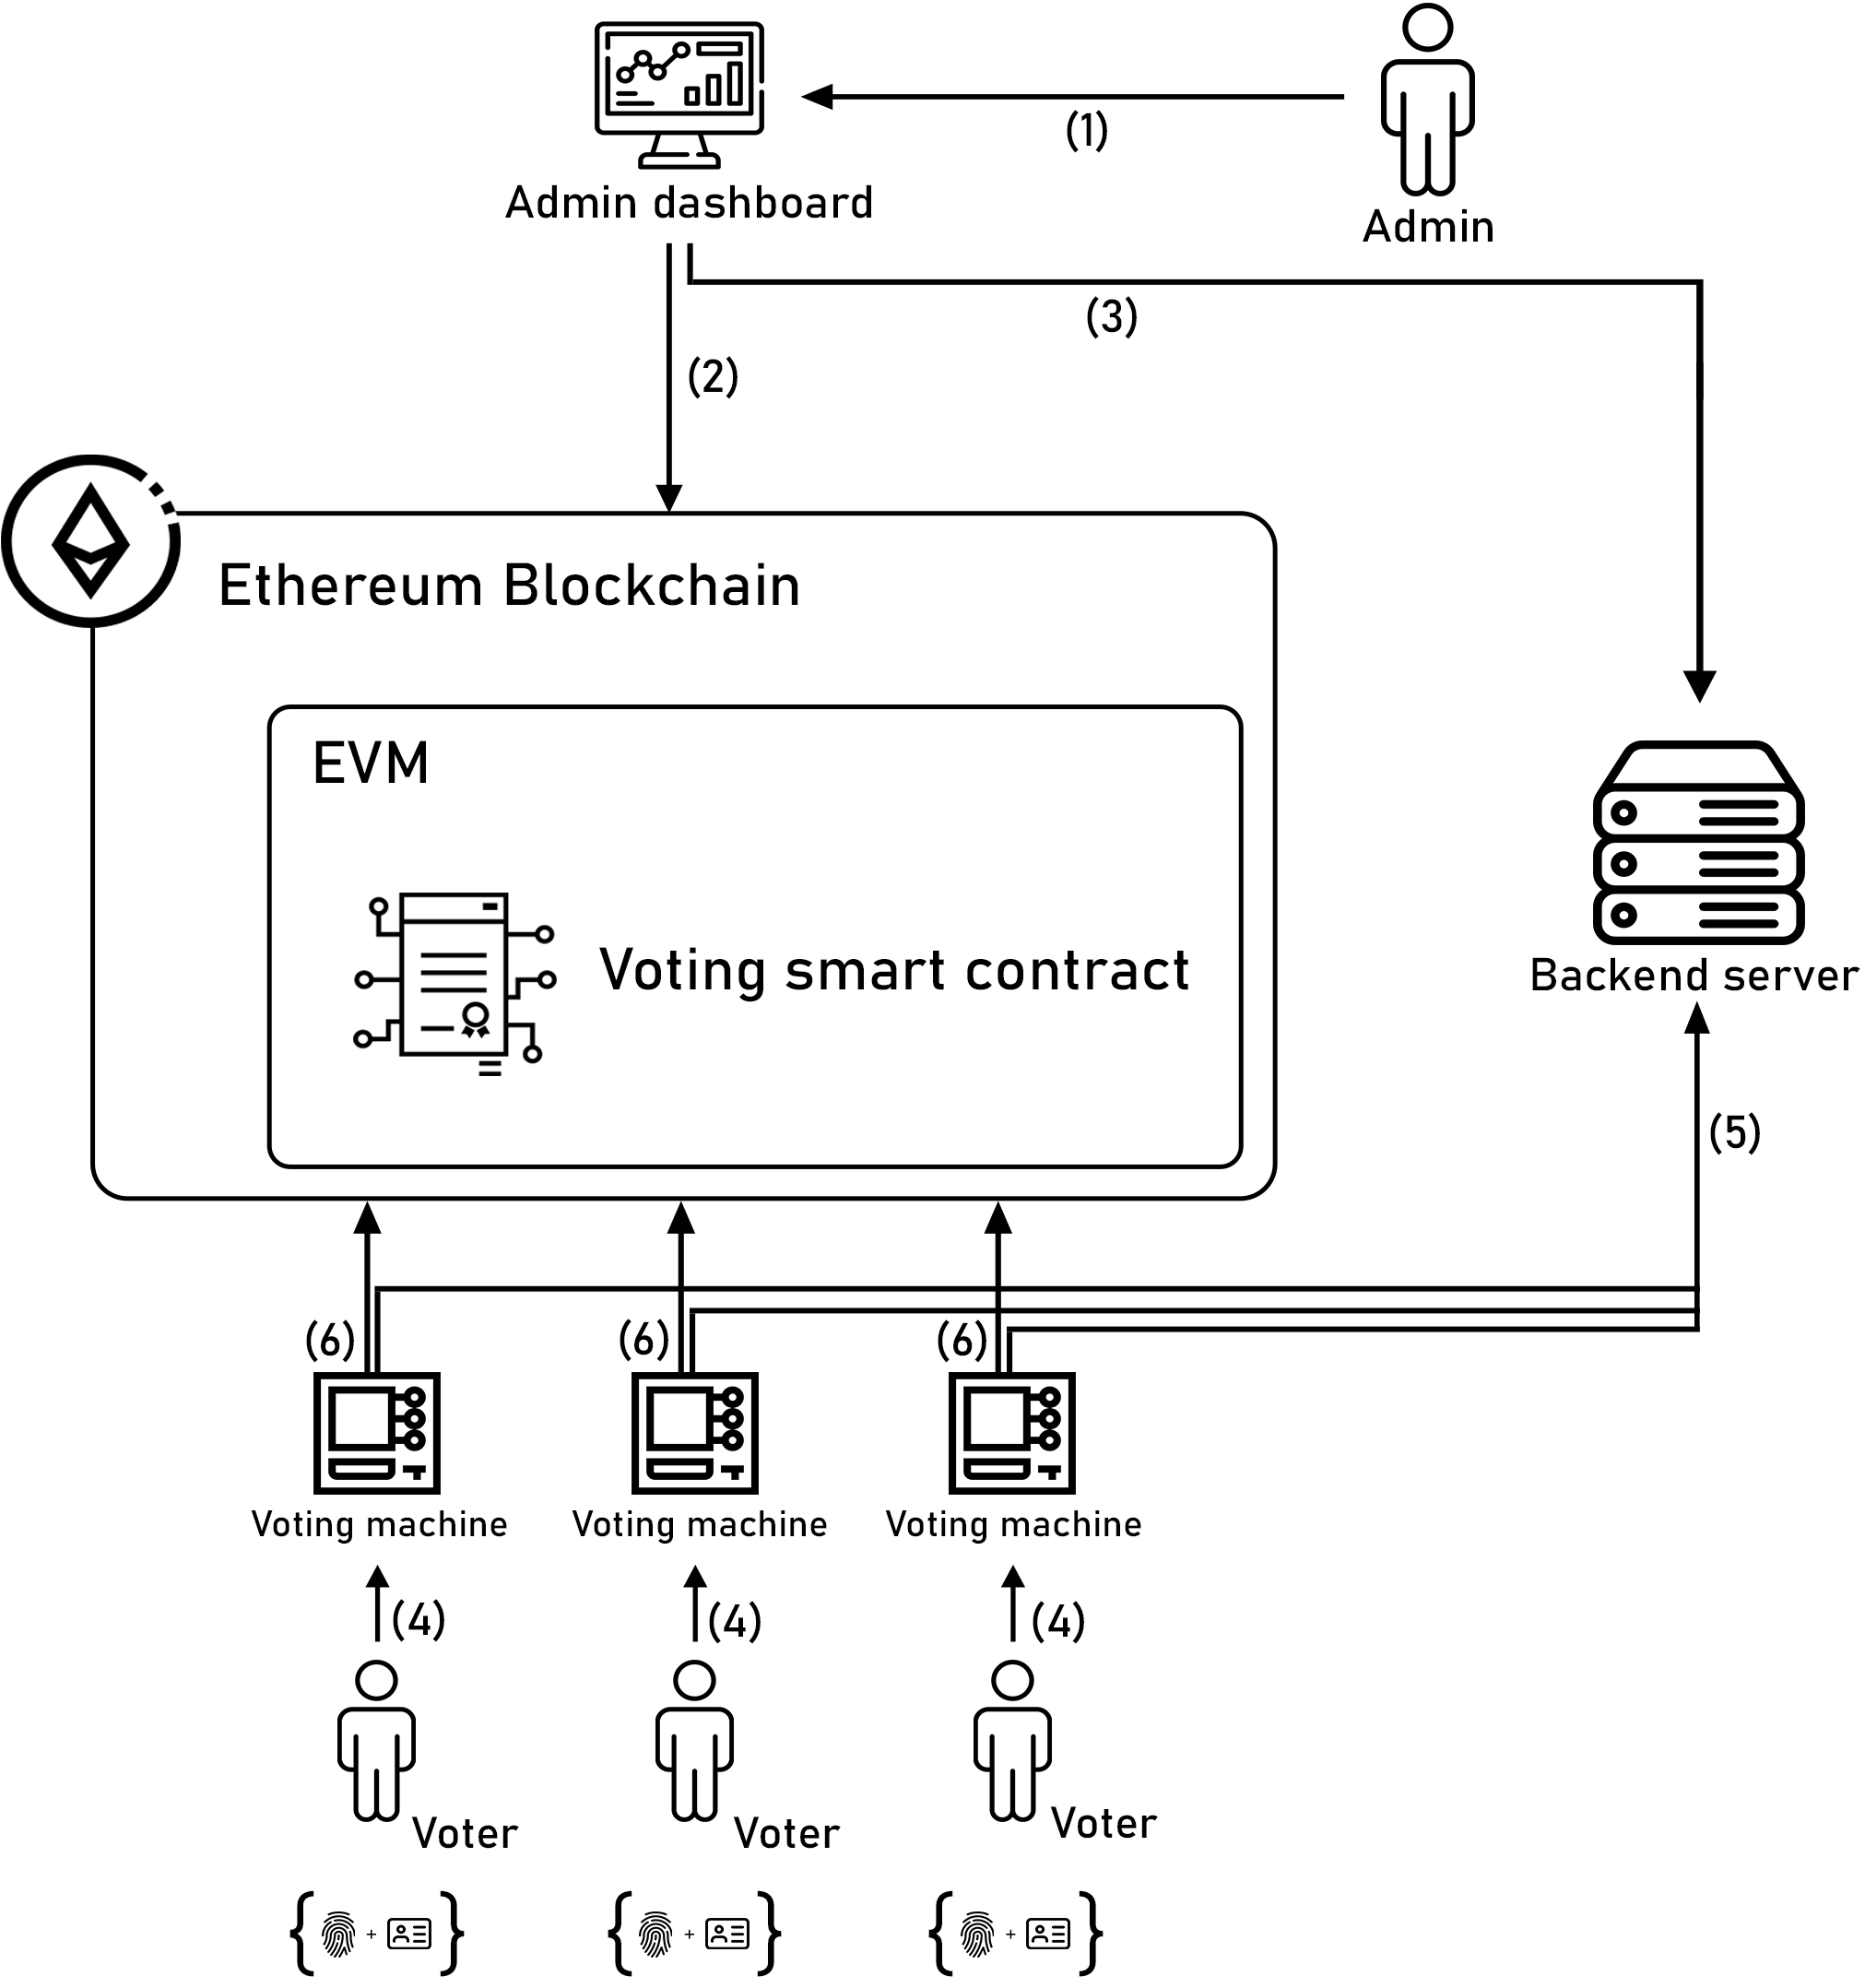
\includegraphics[width=12cm]{images/chapter3/architecture.png}
		\caption{{\footnotesize High level architecture of the proposed system and the interaction between its components}}
\end{figure}

\begin{list}{}{}
\item \textbf{(1)} The admin operating the dashboard launches and monitors voting events
\item \textbf{(2)} Essential data (candidates name and id, event title, start \& finish dates) are saved in the blockchain along with the list of authorized accounts that can interacte with the smart contract.
\item \textbf{(3)} Secondary data that is of less importance is saved to the regular (centralized) backend server.
\item \textbf{(4)} Voters authenticate themselves to the polling machines (using biometric means) and cast their vote to a candidate of their choosing
\item \textbf{(5)} Voting machines uses the backend server to verify the identity of the voter and to fetch secondary data required for the displaying of candidates
\item \textbf{(6)} Voting machines saves the submitted choice to the blockchain by launching a transaction that increments the vote count of the chosen candidate
\end{list}

\subsection{Diagrams}
\subsubsection{Admin sequence diagram}

\begin{figure}[H]
	\centering
		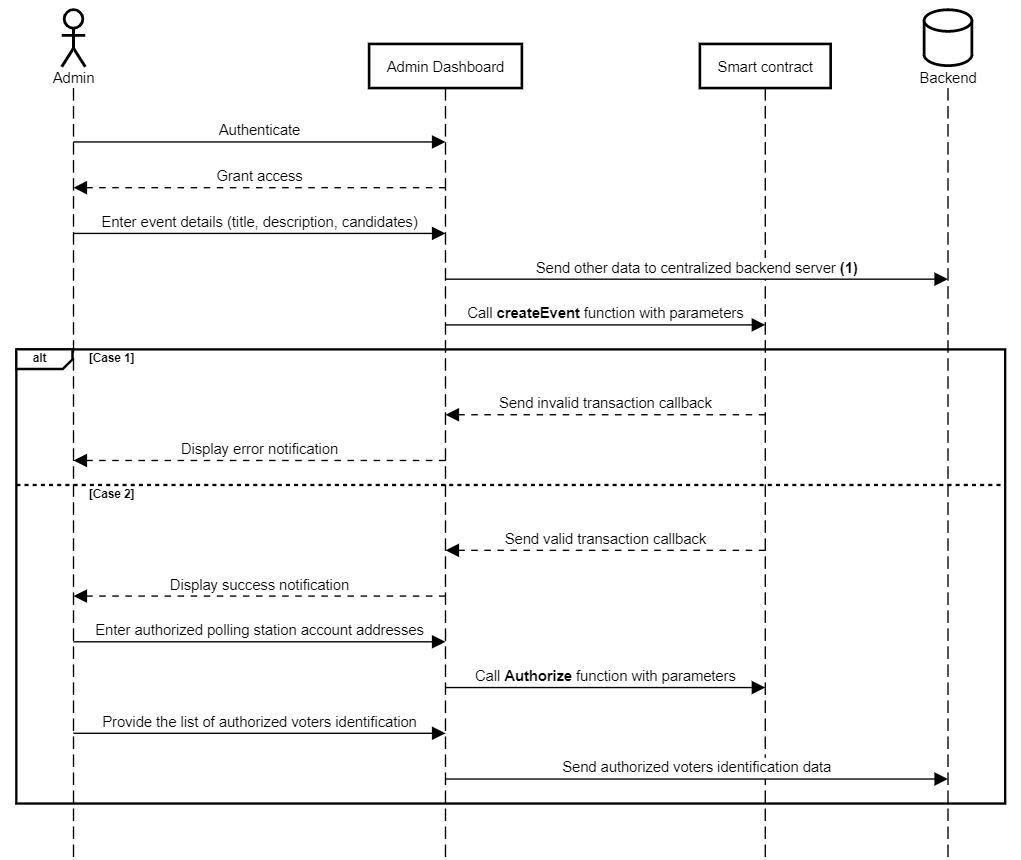
\includegraphics[width=14cm]{images/chapter3/admin_sequence_diagram.png}
		\caption{{\footnotesize Sequence diagram of the process of creating and launching a new voting event}}
\end{figure}

Launching an election requires that the administrator get access to the administration dashboard which has its access restricted by digital or physical boundaries or both, using the dashboard the adminstrator accesses the event creation form, in which he fills the information for the event. The information provided will be divided on the basis of their level of criticality, for example, candidates pictures and lengthy descriptions are deemed to be less critical to the vote counting so they're stored in a regular backend server. Also information required for the authentication of voters is also stored on the regular backend servers.

Next, the administrator is tasked with providing the account addresses of the ethereum accounts running on each voting machine, this list will be the list of the ethereum account addresses allowed to interacte with the smart contract and alter the vote count of any candidates by incrementing it.

\subsubsection{Voter sequence diagram}

\begin{figure}[H]
	\centering
		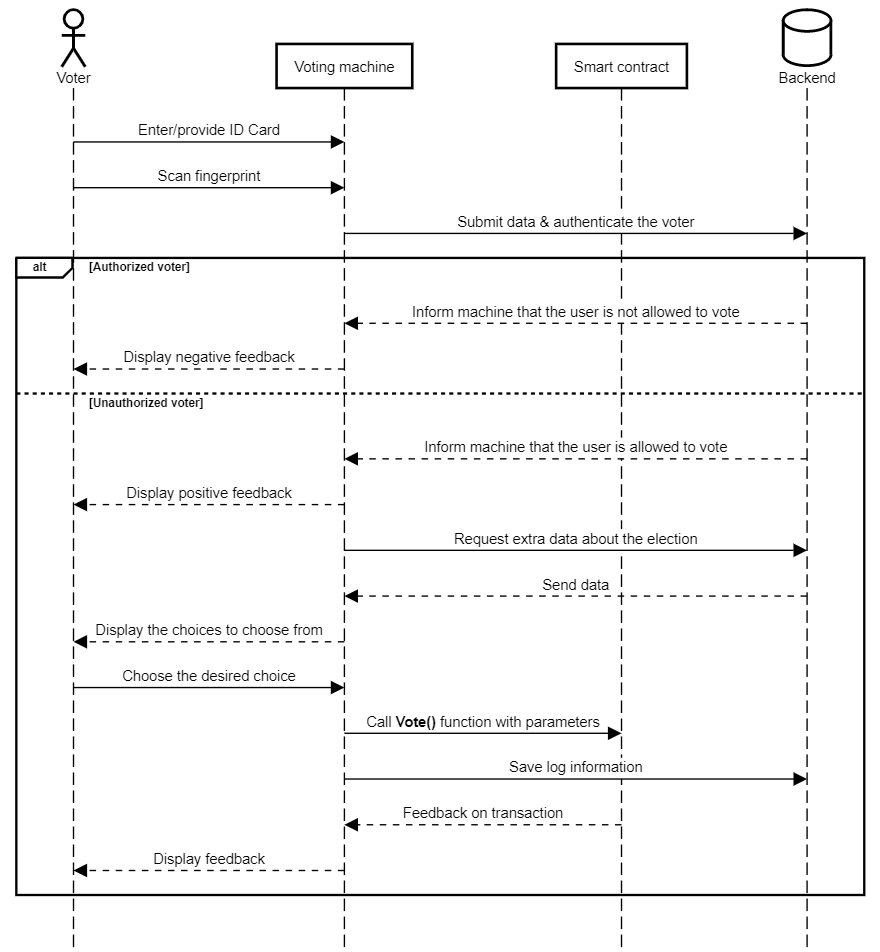
\includegraphics[width=14cm]{images/chapter3/voter_sequence_diagram.png}
		\caption{{\footnotesize Sequence diagram of the process of casting a vote}}
\end{figure}

The process of casting a vote is initiated when a voter first enters a polling station, then proceeds to a vacant voting machine, the machine should be equipped with ID Card reader and fingerprint scanner to conduct a biometric identity check. the information obtained will be checked against the records saved on the backend server. In case the person is identified as an authorized voter; meeting whataver the requirements listed by the entity organizing the voting event (for example an entity can enforce one single vote per a household or set the minimum age for participation to 50), a list of choices will be displayed to the voter to choose from in a intuitive manner, after the voter makes his choice and submits it, the voting machine performance an ethereum transaction to the smart contract by calling the appropriate function that will result in incrementing the vote count of that particular candidate, also log information about the vote will be saved to the backend server.

\section{Results}

In this section we will go through the results that were obtained by this investigatory efforts and showcase the various components of the proof-of-concept that was developed.

\subsection{Admin dashboard}

\begin{figure}[H]
	\centering
		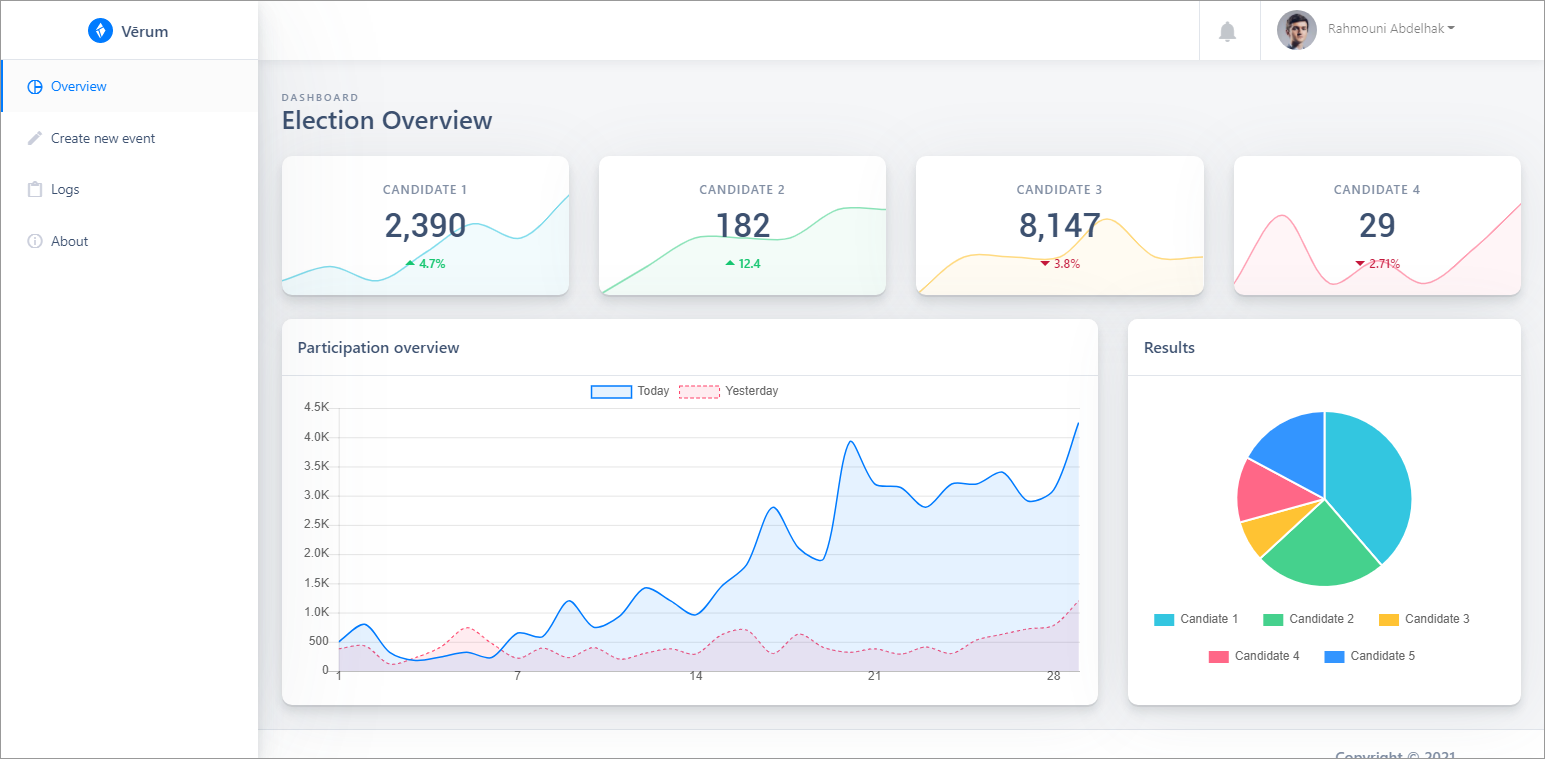
\includegraphics[width=14cm]{images/chapter3/admin_1.png}
		\caption{{\footnotesize Election overview tab of admin dashboard}}
\end{figure}

\begin{figure}[H]
	\centering
		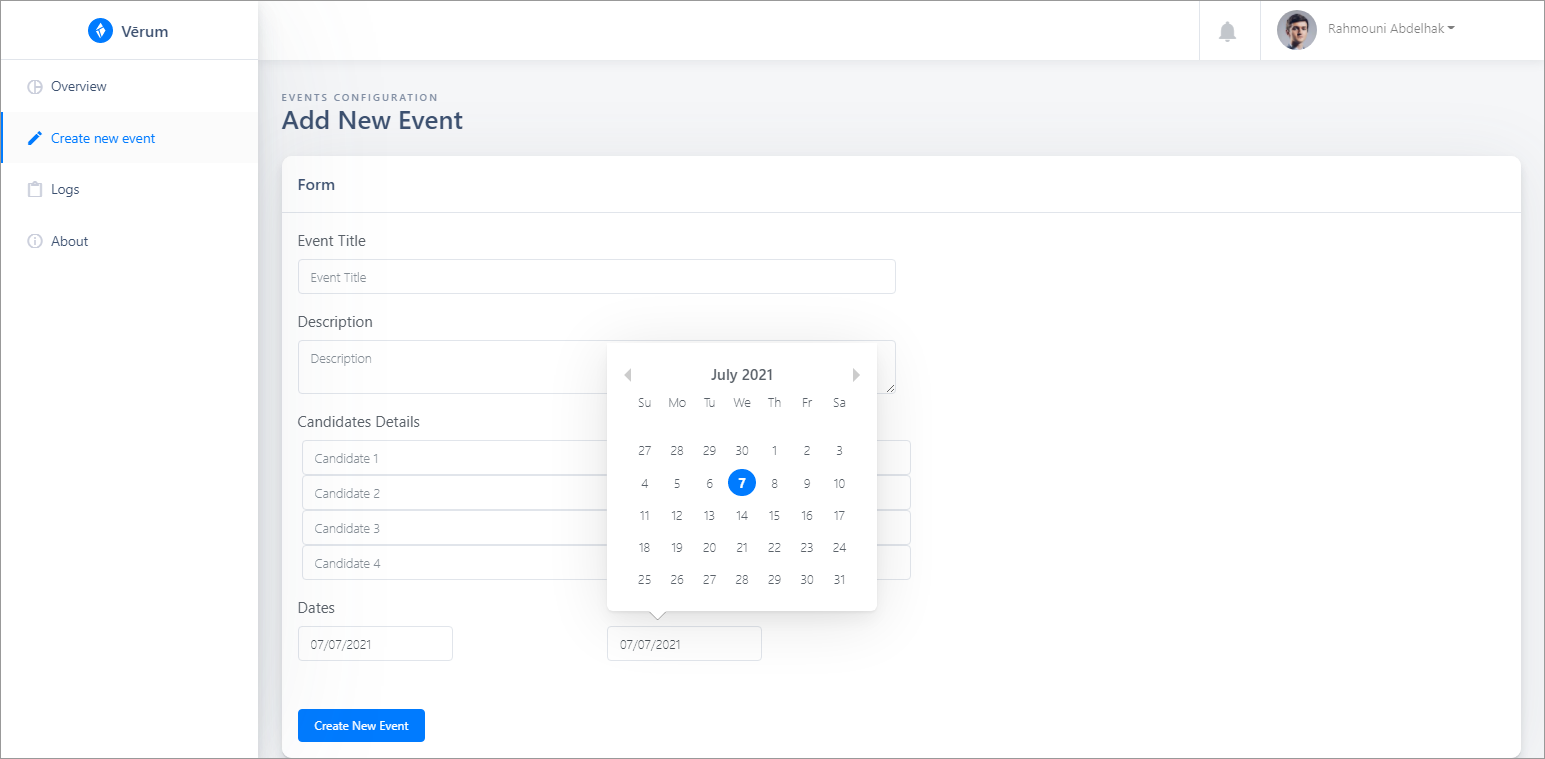
\includegraphics[width=14cm]{images/chapter3/admin_2.png}
		\caption{{\footnotesize Event creation tab of the admin dashboard}}
\end{figure}

\begin{figure}[H]
	\centering
		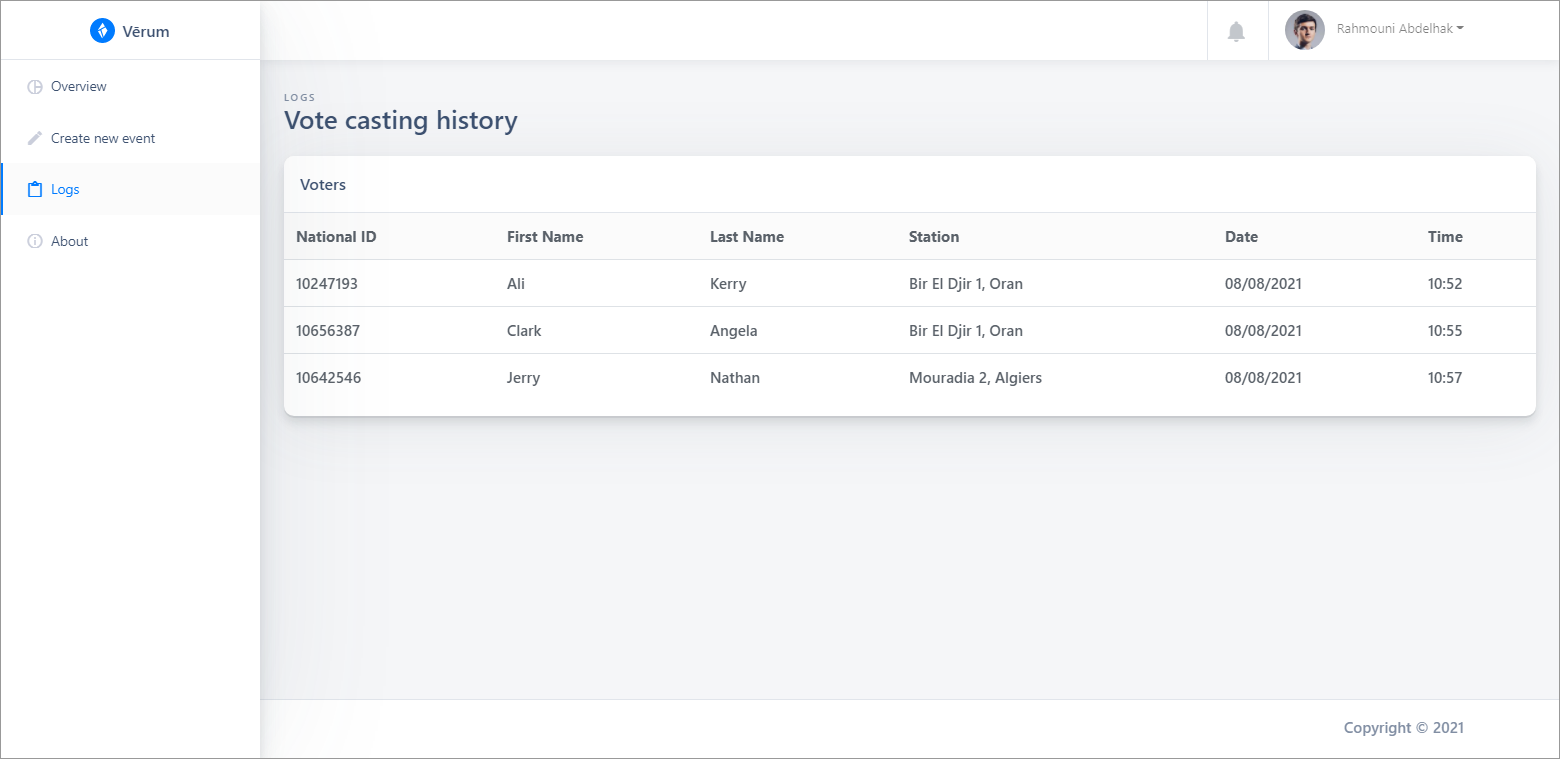
\includegraphics[width=14cm]{images/chapter3/admin_3.png}
		\caption{{\footnotesize Logs tab of the admin dashboard}}
\end{figure}

\subsection{End-user (voter) application}

\begin{figure}[H]
	\centering
		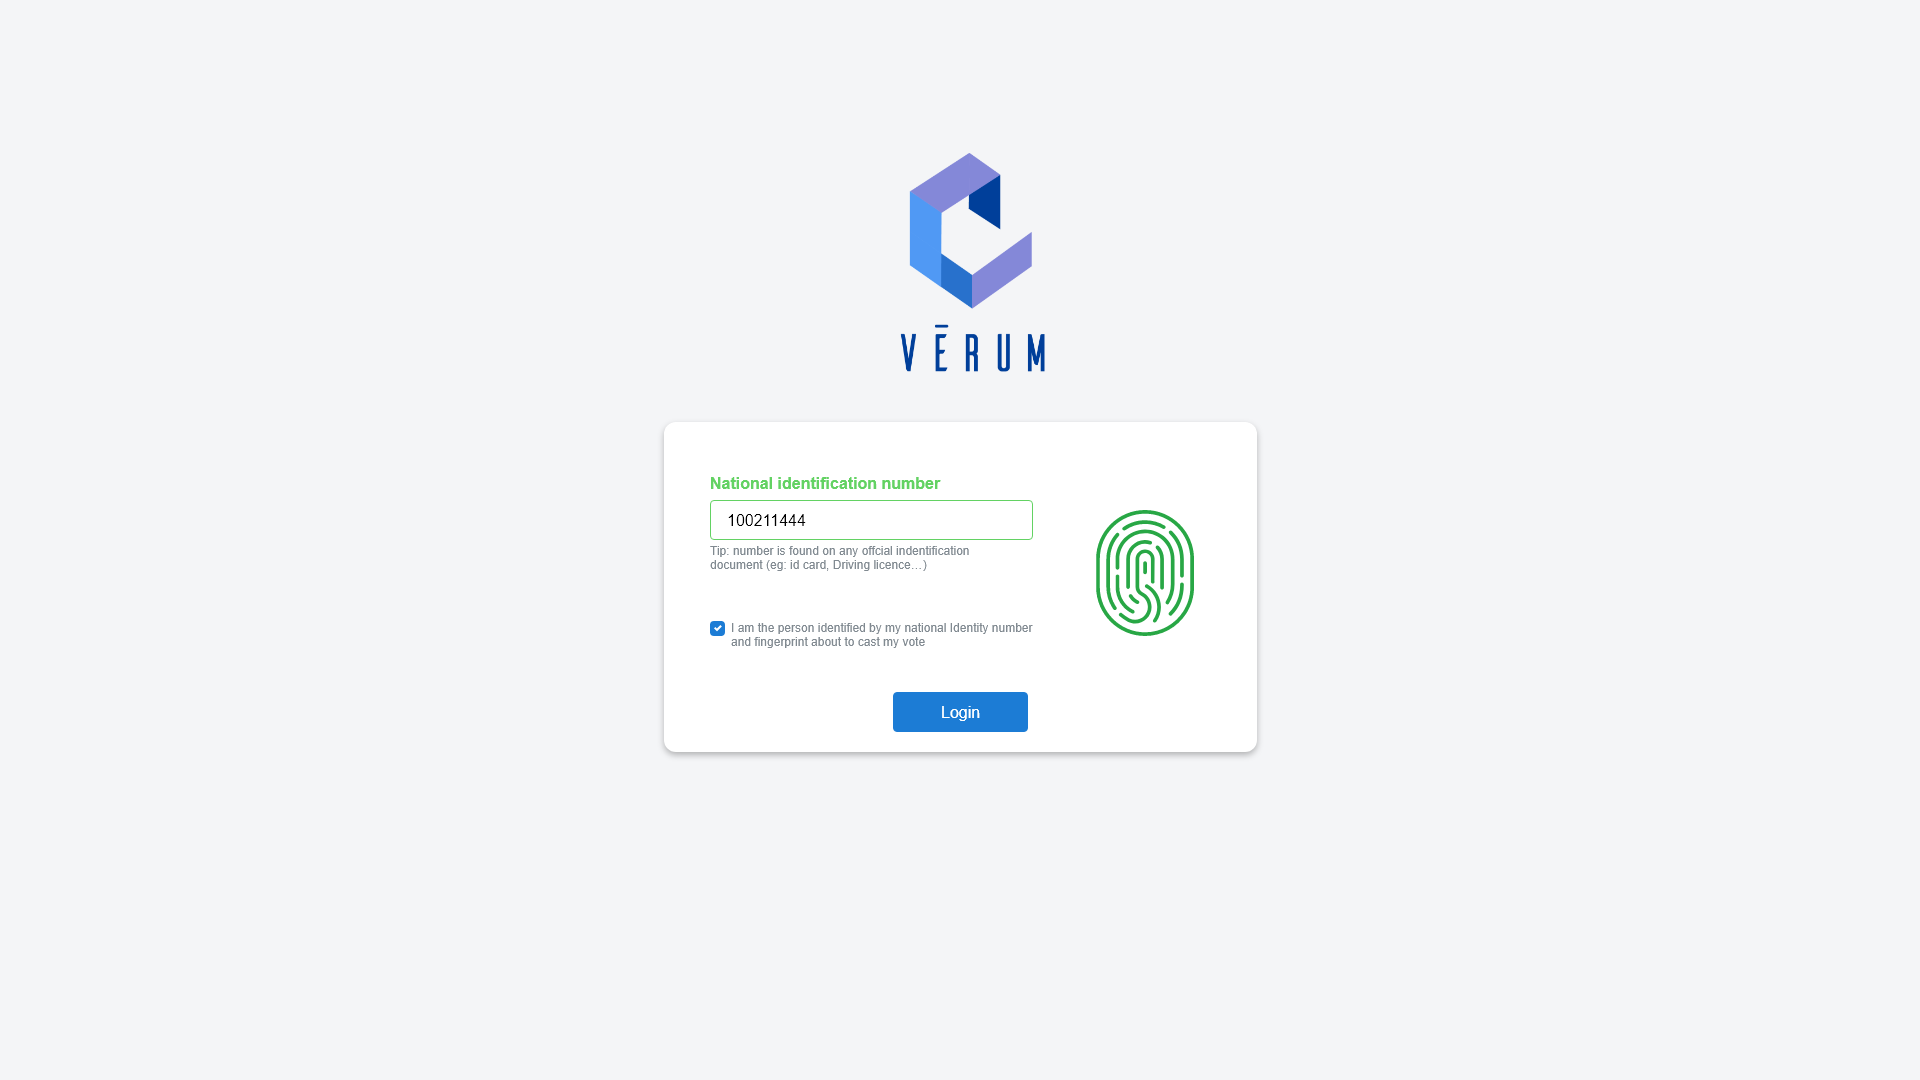
\includegraphics[width=14cm]{images/chapter3/voter_2.png}
		\caption{{\footnotesize Election overview tab of admin dashboard}}
\end{figure}

\begin{figure}[H]
	\centering
		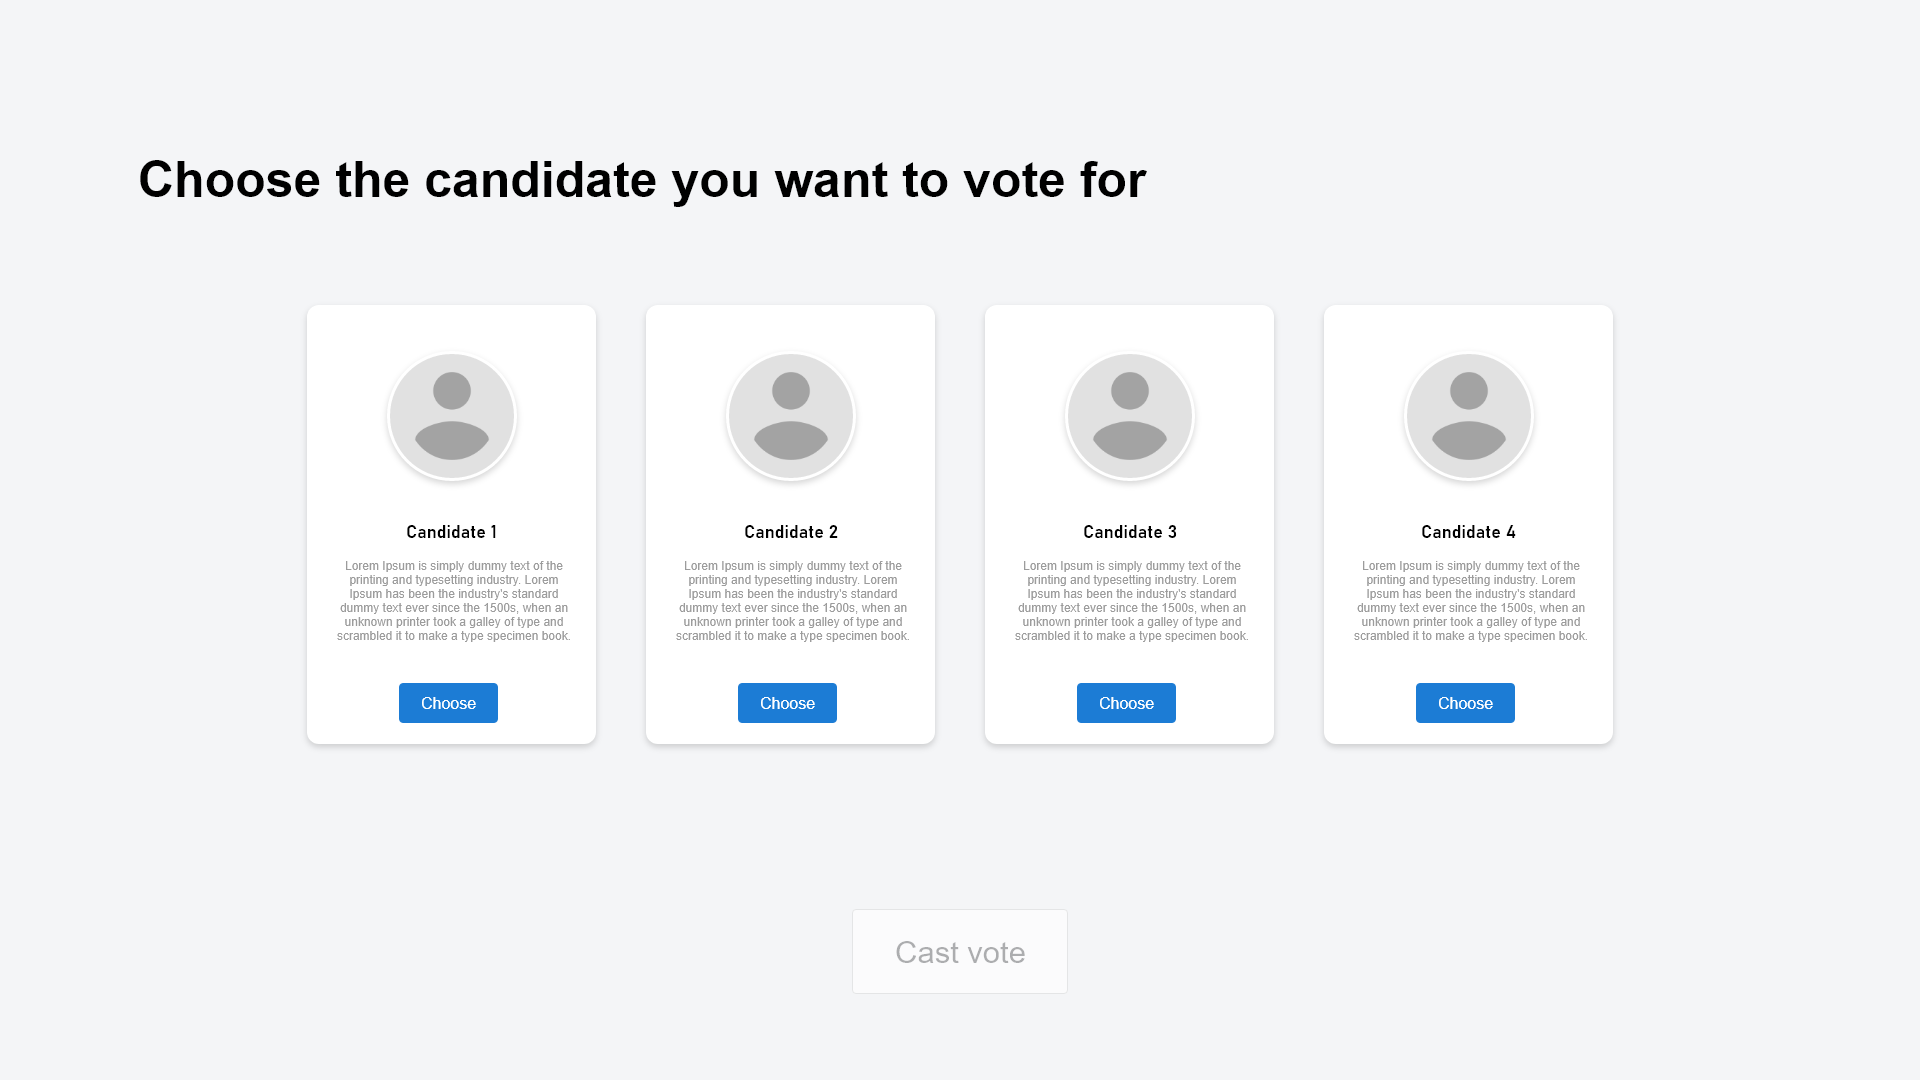
\includegraphics[width=14cm]{images/chapter3/voter_3.png}
		\caption{{\footnotesize Event creation tab of the admin dashboard}}
\end{figure}

\begin{figure}[H]
	\centering
		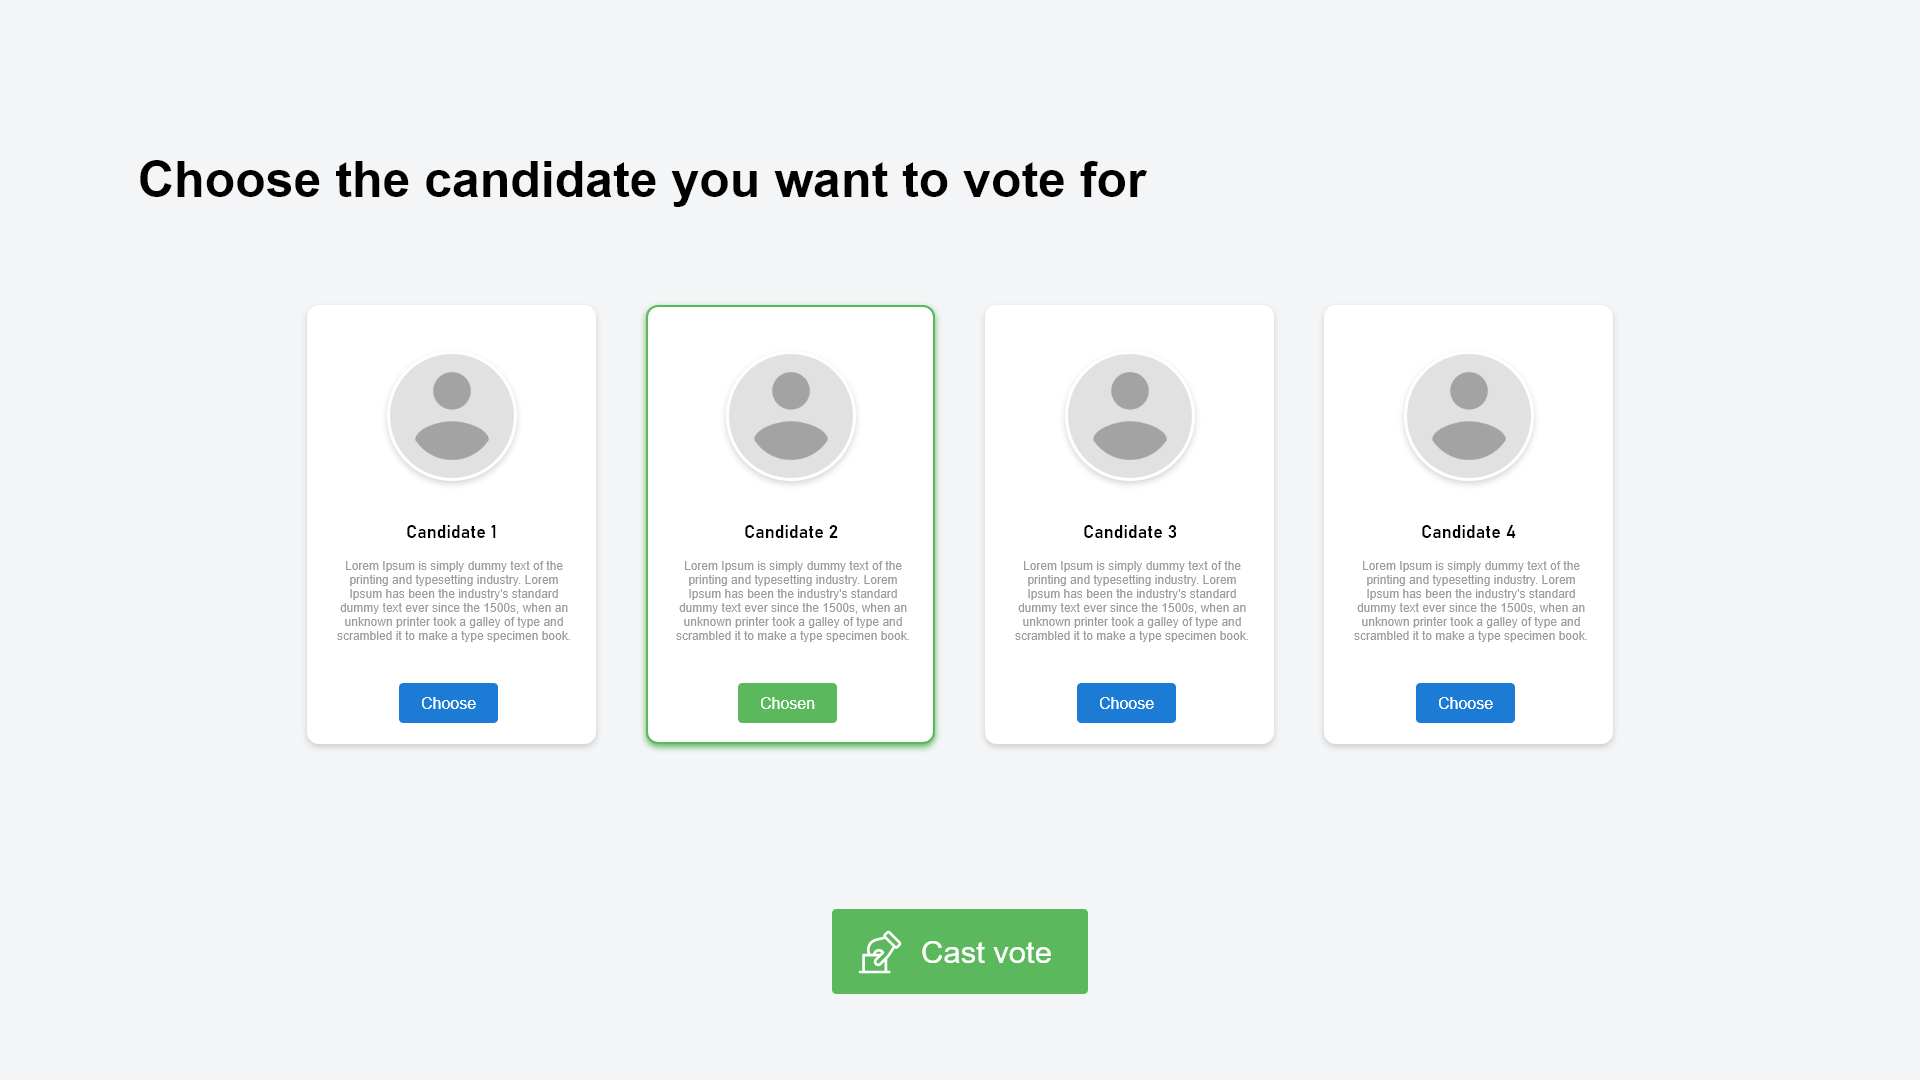
\includegraphics[width=14cm]{images/chapter3/voter_4.png}
		\caption{{\footnotesize Logs tab of the admin dashboard}}
\end{figure}

\begin{figure}[H]
	\centering
		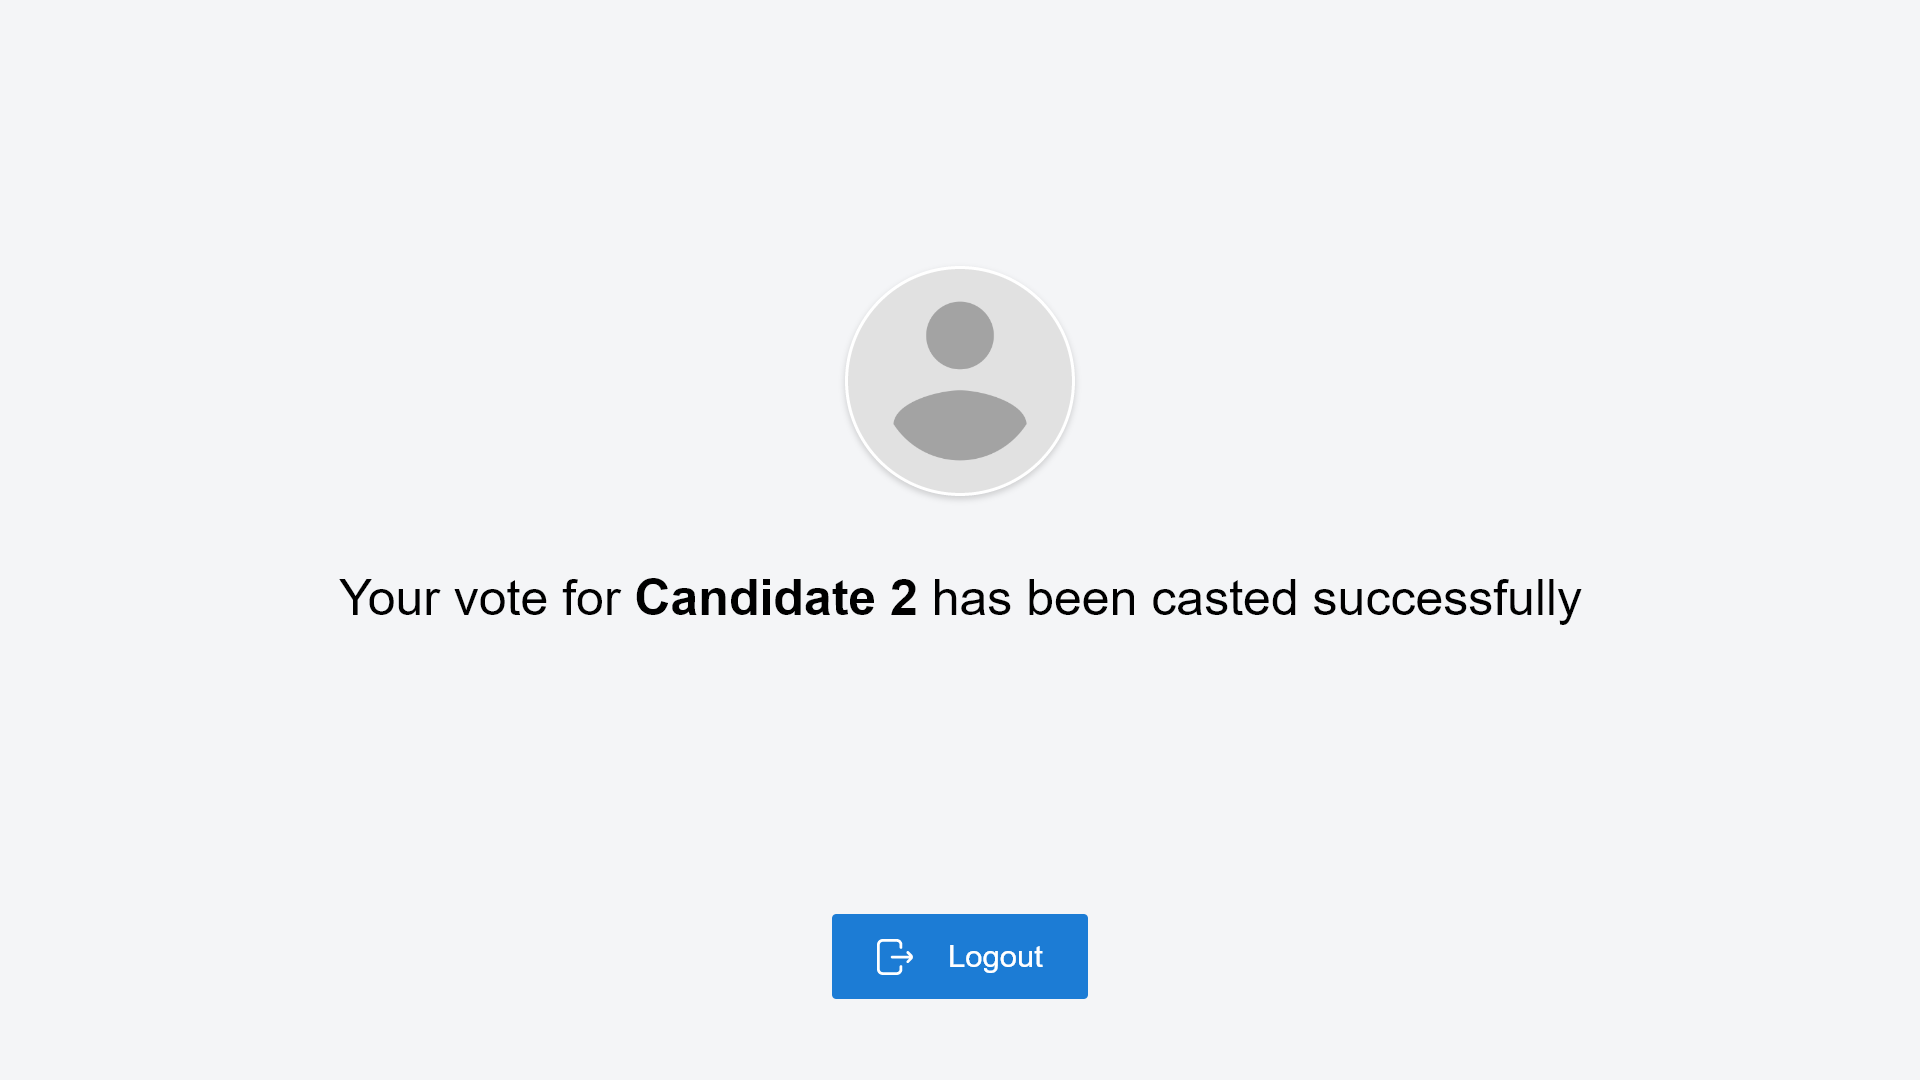
\includegraphics[width=14cm]{images/chapter3/voter_5.png}
		\caption{{\footnotesize Logs tab of the admin dashboard}}
\end{figure}
\newpage

\subsection{Smart contract}

\begin{figure}[H]
	\centering
		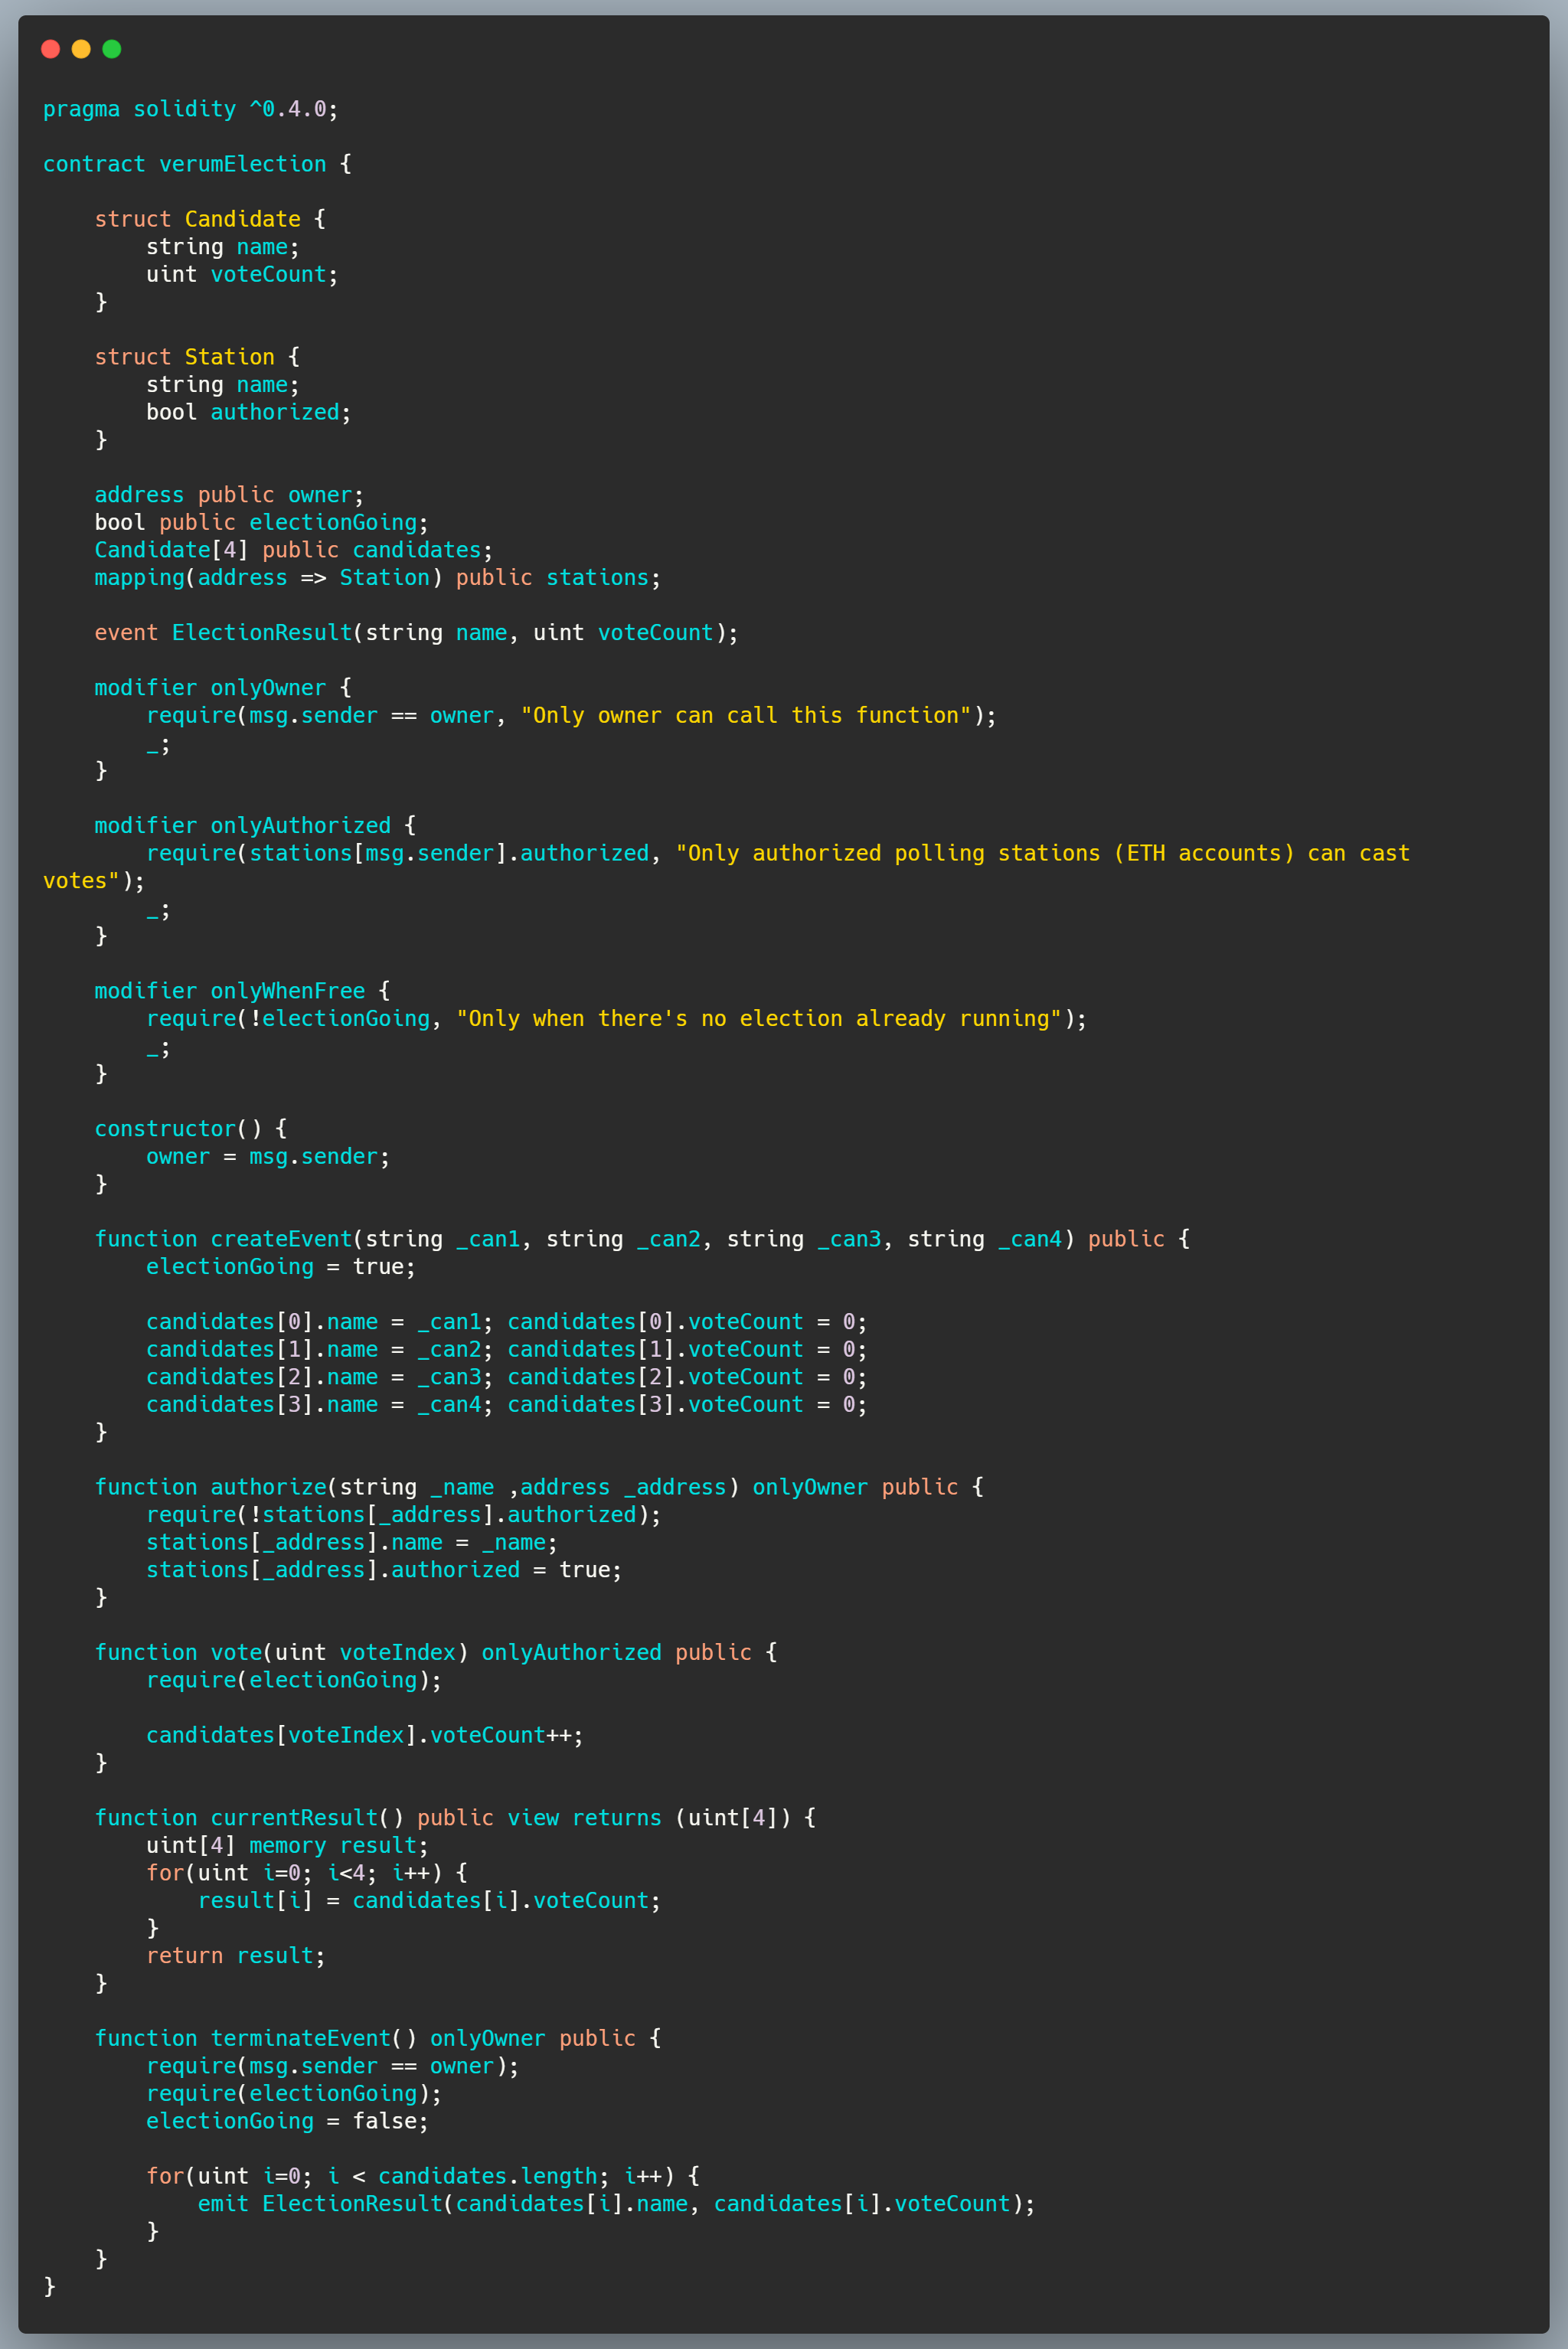
\includegraphics[width=12cm]{images/chapter3/smart-contract.png}
		\caption{{\footnotesize Voting smart contract written in solidity language}}
\end{figure}

\subsection{Tests}
To ensure the proof-of-concept built actually delivered the results we initially intended to achieve a few tests were conducted.


